
\section{Statistical Inference}
\begin{frame}{What is Statistical Inference?}
  \begin{block}{}
    {\bf Statistical inference} is the process of using data analysis to deduce properties of an underlying statistical distribution.
  \end{block}\bigskip
  \begin{columns}
    \column{.3\textwidth}
      \includegraphics[width=\textwidth]{../img/sampling_distribution}
    \column{.7\textwidth}
      Remember that a sample from a distribution is a \emph{random variable}, defined by a \emph{sampling distribution}. \medskip

      The sampling distribution is characterized by parameters from the distribution. So when we deduce properties of the sampling distribution, we can use these properties to characterize the underlying population.
  \end{columns}\bigskip

  \begin{center}
  Sample data $\rightarrow$ Sampling distribution $\rightarrow$ Population parameters
  \end{center}
\end{frame}

\subsection{Statistical Hypothesis}
\begin{frame}{What is a hypothesis?}
  A key tool of statistical inference is the {\bf Statistical Hypothesis}:
  \begin{block}{Many meanings of hypothesis}
    {\bf Hypothesis:} a proposed explanation to an observable phenomenon.\\
    {\bf Scientific Hypothesis:} must be \emph{Testable} and \emph{Falsifiabe};\\
    {\bf Statistical Hypothesis:} explanation focus on statistical statements;\\

  \end{block}\bigskip

  \begin{columns}
    \column{0.8\textwidth}
    {\bf Example:} Your cocoa factory is working normally, so the mean of its production is \emph{no less than 300g}.
    \begin{itemize}
      \item {\bf Testable}: analyze a produced sample;
      \item {\bf Falsifiable}: estimated mean is \alert{much below 300g}
    \end{itemize}
    \column{0.2\textwidth}
    
\includegraphics[width=\textwidth]{../img/irasutoya_cocoa}
  \end{columns}
  \vfill

  Key question: how much is "\emph{much below 300g}"?
\end{frame}

\begin{frame}{Comparing Multiple Hypotheses}
  In general we can propose several hypothesis for the same observation. We  compare these hyposeses against each other, and try to decide which one is {\bf more likely to be true} based on the data.

  \begin{block}{Cocoa Sample (sample mean: 294)}
    293 325 \alert{271} 313 309 298 284 304 \alert{248} 296\\
  \end{block}\bigskip

  Hypotheses:
  \begin{itemize}
    \item Sample mean under 300 is bad luck. Factory mean is $\approx$ 300g.
    \item Factory mean is than 300g. Factory has a problem.
    \item An evil employee sabotaged the sample, choosing bad packages.
    \item The balance I used to measure the sample is broken.
    \item Factory production depends on the hour of the day.
  \end{itemize}
\end{frame}

\begin{frame}{Comparing Multiple Hypotheses}{Comparison criteria}
  When comparing multiple hypothesis, we want to keep several criteria in mind:
  \begin{itemize}
    \item {\bf Predictive power}: The hypothesis allows you to predict future behavior of the system.\medskip
    \item {\bf Principle of parsimony} (Ockham's razor): The hypothesis makes few assumptions about the system.\medskip
    \item {\bf Fitting the data}: The data supports the hypothesis and has a high probability of being produced under it.\medskip
    \item {\bf External consistency}: The hypothesis fits with existing, well accepted knowledge about the system.\medskip
  \end{itemize}
\end{frame}

\begin{frame}{Multiple hypotheses and statistical testing}
  One way that we compare multiple hypotheses is by calculating the probability of the observed sample under each competing hypothesis. In this sense, we give more credibility for the hypothesis that maximizes the probability of the observed sample.\bigskip

  \begin{itemize}
    \item $P(\bar{x}|H_1), P(\bar{x}|H_2), P(\bar{x}|H_3), \ldots$
  \end{itemize}\bigskip

  \begin{columns}
    \column{0.4\textwidth}
    \begin{block}{Hypothesis 1: $\mu \geq 300$}
      What is the probability that we see the sample: $X = \{293, 325, 271, 313, \ldots\}$ when the mean production of the factory is at least 300g?
    \end{block}
    \column{0.2\textwidth}
    
\includegraphics[width=\textwidth]{../img/irasutoya_cocoa}
    \column{0.4\textwidth}
    \begin{block}{Hypothesis 2: $\mu < 300 - \delta$}
      What is the probability that we see the sample: $X= \{293, 325, 271, 313, \ldots\}$ when the mean production of the factory is much lower than 300g?
    \end{block}
  \end{columns}

\end{frame}



\begin{frame}{Null and alternate hypothesis}
  The \emph{Null Hypothesis Significance Testing (NHST)} approach involves the contrast between a {\bf null hypothesis} and an {\bf alternative hypothesis}.\bigskip

  \begin{columns}
    \column{0.5\textwidth}
    \begin{block}{Null Hypothesis ($H_0$)}
      \begin{itemize}
        \item Absence of effects;
        \item Conservative model;
        \item "nothing special is happening"
      \end{itemize}
      \bigskip

      "The mean production of the chocolate factory is at least 300g"
      \bigskip

      {\bf $H_0: \mu \geq 300$}
    \end{block}
    \column{0.5\textwidth}
    \begin{block}{Alternative Hypothesis ($H_1$)}
      \begin{itemize}
        \item Presence of some effect;
        \item Something "new" is happening;
      \end{itemize}
      \bigskip

      "For \alert{some reason}, the mean production is below 300g"
      \bigskip

      {\bf $H_1: \mu < 300$}
    \end{block}
  \end{columns}
\end{frame}

\begin{frame}{Null Hypothesis Testing}{How to choose a null hypothesis?}
  \begin{itemize}
    \item Use existing knowledge about the process being investigated;
    \item Values obtained from theory or models (model validation);
    \item System requirements (investigation of system compliance);
  \end{itemize}
  \bigskip
  \begin{block}{Chocolate factory example:}
    We suspect that there may be a problem in our chocolate production. We propose sampling $20$ packages, and estimating the \emph{mean} of the population from this sample:
    \bigskip
    \begin{itemize}
      \item {\bf Null Hypothesis:} $H_0: \mu \geq 300$
      \item {\bf Alternative Hypothesis:} $H_1: \mu < 300$
    \end{itemize}
  \end{block}
\end{frame}


\begin{frame}{Null Hypothesis Testing}{Testing Assumptions}
  Notice that the \emph{NHST} approach adpts a number of assumptions, both statistical and technical:\bigskip

  \begin{itemize}
    \item The mean is a good measure for the question of interest.\\
    (i.e., the variance of production is small enough, the weigths of items are indepentent, customers usually purchase many packages, so individual extreme values are not important, etc);\bigskip

    \item The packages sampled are representative of our population of interest (i.e., the packages are from regular production (not specially produced for this test), they are not tampered with, etc)\bigskip

    \item The contents of the packages are actually chocolate (the weight of the package is not a significant part of the measured weight, etc);\bigskip

    \item etc ...
  \end{itemize}
\end{frame}

\begin{frame}{Null Hypothesis Testing}{Testing Procedure}
  \begin{enumerate}
    \item Obtain a sample (i.e. running the experiment);
    \item Calculate test statistics from the sample data;
    \item Make a decision based on the computed value;
  \end{enumerate}\medskip

  As the sample mean ($\bar{X}$) is a good estimator for the population mean ($\mu$), the decision to reject or not the null hypothesis could be made based on the difference $\Delta$ between the sample mean and $\mu_{H_0}$.\medskip

  But how do we define this {\bf critical region} for rejecting $H_0$?

  \begin{center}
    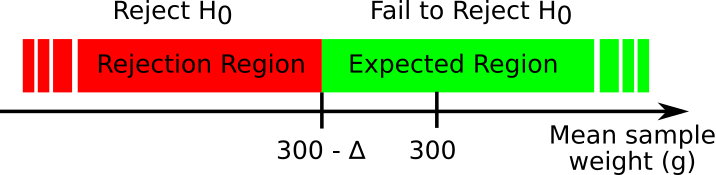
\includegraphics[width=.8\textwidth]{../img/critical_region}
  \end{center}

\end{frame}



\subsection{Inference Errors}
\begin{frame}{Inference Errors}
  Remember that a parameter estimator from a sample is a random variable, with an {\bf estimator error} associated with it. Because of this, there is a chance that the hypothesis test reaches a \alert{wrong conclusion}.\bigskip

  \begin{itemize}
    \item If the estimatior error is too large, the sample mean could be in the rejection region, even if the null hypothesis is true;\medskip
    \item If $\Delta$ is too large, the sample mean could be in the expected region, even if the null hypothesis is not true;
  \end{itemize}\bigskip

  We want to be able to estimate (and control!) the probability of these errors.

  \begin{center}
    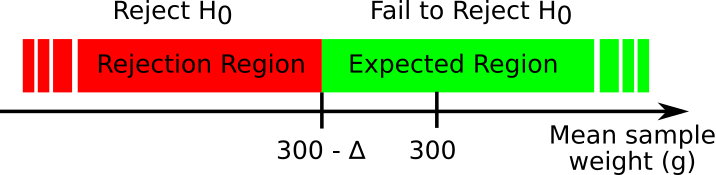
\includegraphics[width=.8\textwidth]{../img/critical_region}
  \end{center}
\end{frame}

\begin{frame}{Type I Error}
  \begin{block}{}
    {\bf Type I Error (False Positive)}:\\
      \hspace{1cm}Reject the Null Hypothesis when it is true
  \end{block}\medskip

  The probability of occurrence of a false positive in any hypothesis testing procedure is generally known as the \structure{significance level} of the test, represented by the Greek letter $\alpha$:
  \begin{equation*}
    \alpha = P(\text{type I error}) = P(\text{reject }H_0|H_0\text{ is true})
  \end{equation*}
  \bigskip

  Another frequently used term is the \structure{confidence level} of the test, which is given by $(1-\alpha)$ or $100(1-\alpha)$\%
\end{frame}

\begin{frame}{Type I Error}{Choosing $\alpha$ and the rejection region}
  For a given sample, the value selected for $\alpha$ defines the threshold for the rejection of $H_0$. If $H_0$ is true (i.e., $\mu = 300$g), we can expect that the distribution of mean estimates is approximately normal\footnote{Assuming the CLT conditions are met}, with average 300g and standard error $(\sigma/\sqrt{n})$.
  \vspace{1cm}

  \begin{columns}
    \column{0.5\textwidth}
    To control the probability of Type I error (e.g. $\alpha=0.05$), we select the critical region so that the cumulative probability under the distribution of $\hat{x}$ inside that region is $1-\alpha=0.95$.
    \column{0.5\textwidth}
    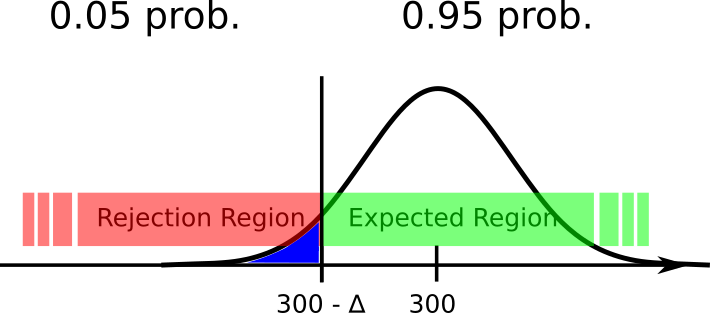
\includegraphics[width=\textwidth]{../img/critical_region_alpha}
  \end{columns}
\end{frame}

\begin{frame}{Type II Error}
  \begin{block}{}
    {\bf Type II Error (False Negative):}\\
    \hspace{1cm} Fail to reject the Null Hypothesis when it is false
  \end{block}
  \bigskip

  The probability of occurrence of a false negative in any hypothesis testing procedure is generally represented by the Greek letter $\beta$:
  \begin{equation*}
    \beta = P(\text{type II error}) = P(\text{not reject }H_0|H_0\text{ is false})
  \end{equation*}\bigskip

  The quantity $(1 - \beta)$ is known as the \structure{power} of the test. It quantifies the test's sensitivity to effects that violate the null hypothesis.
\end{frame}

\begin{frame}{Type II Error}{Interpretation}
  \begin{columns}
    \column{.6\textwidth}
    Unlike the Type-I error, the definition of the error rate for the Type-II error requires the specification of the value of the parameter of interest under the alternative hypothesis.
    \bigskip

    The probability of failing to reject a false $H_0$ strongly depends on the magnitude of the difference between the value of the parameter under $H_0$ and the real value of the parameter.
    \column{.4\textwidth}
    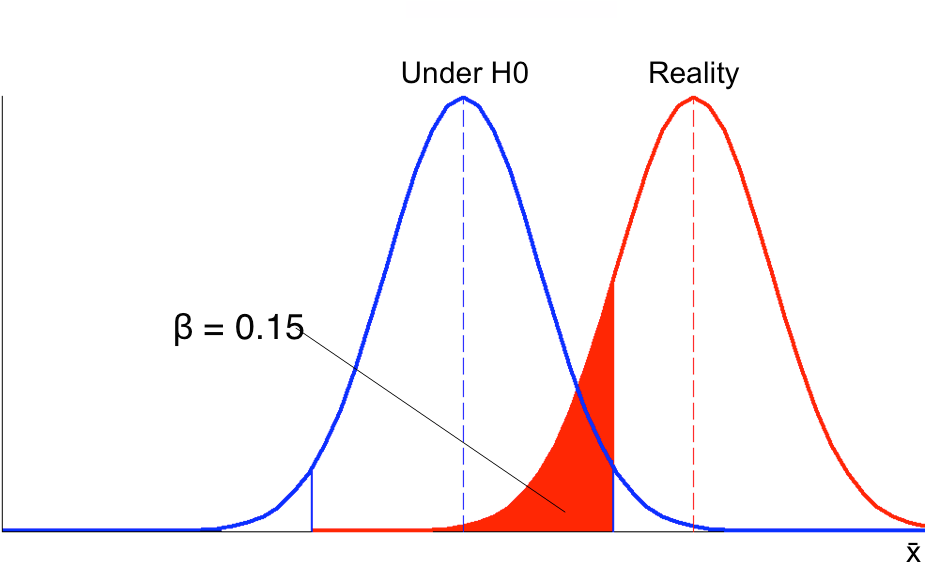
\includegraphics[width=\textwidth]{../img/beta-a}\\
    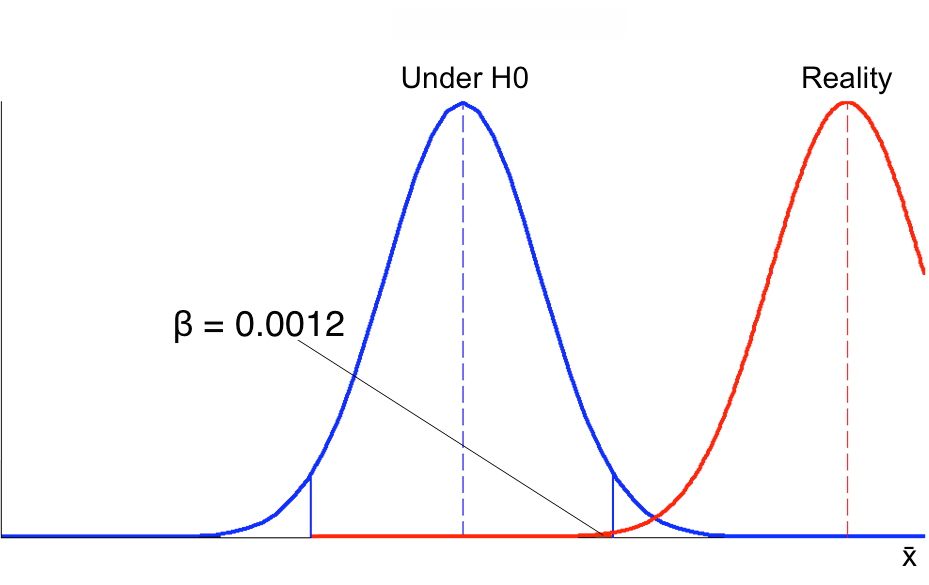
\includegraphics[width=\textwidth]{../img/beta-d}
  \end{columns}
\end{frame}

\begin{frame}{Type II Error}{Controlling $\beta$}
  The power $\beta$ of a test is governed by several factors:
  \begin{itemize}
    \item {\bf Controllable}: significance level, sample size;
    \item {\bf Uncontrollable}: real value of the parameter, variance;
  \end{itemize}\bigskip

  If $H_0$ is false, a smaller magnitude of the difference between the real value of the parameter and the one under the null hypothesis leads to a greater probability of a type II error. {\bf On the other hand, the practical importance of the error gets smaller.}\vfill

  In general, it is possible to estimate the power of a test for target desired differences $|H_0 - H_1|$.
\end{frame}

\begin{frame}{Considerations on Inference Errors}

  {\bf Type I Error} $(\alpha)$: depends only on the distribution of the null hypothesis -- easier to control;\\
  {\bf Type II Error} $(\beta)$: depends on the real value of the parameter -- more difficult to specify and control;\\
  \bigskip

  These characteristics lead to the following classification of the conclusions obtained from a test of hypotheses:
  \begin{exampleblock}{}
    \begin{itemize}
      \item Rejection of $H_0$ - strong conclusion;
      \item Failure to Reject $H_0$ - weak conclusion (but we can strengthen it);
    \end{itemize}
  \end{exampleblock}
  It is important to remember that failing to reject $H_0$ does not mean that there is evidence in favor of $H_0$ -- it only suggests that it is a better model than the alternative proposed.
\end{frame}

\subsection{Hypothesis Testing}
\begin{frame}{Hypothesis testing}{General Procedure}
  \begin{enumerate}
    \item Identify the parameter of interest;
    \item Define $H_0$ and $H_1$ (one- or two-sided);
    \item Determined desired $\alpha$ and $\beta$;
    \item Define minimal interesting effect size $\delta^{*}$;
    \item Calculate sample size;
    \item Determine the test statistic and critical region;
    \item Compute the statistic;
    \item Decide whether or not to reject $H_0$;
  \end{enumerate}
\end{frame}

\begin{frame}{Hypothesis Testing Example 1}{Mean of a normal distribution, variance known}
  For a certain brand of peas, we want to determine if there is any significant deviation in the mean weight of sacks from an advertised amount. Assume (for now) that the true variance of the process is known. The test hypotheses are defined as:\medskip

  \begin{itemize}
    \item $H_0: \mu = 50\text{kg}$
    \item $H_1: \mu \neq 50\text{kg}$
  \end{itemize}\medskip

  Let the desired significance level be $\alpha = 0.05$.\medskip

  Given these characteristics, we expect that the sampling distribution of $\bar{X}$ is normal, with Var$(\bar{X})$ = $\sigma^2/n$ and, {\bf if $H_0$ is true}, a mean of $\mu_{\bar{X}} = \mu_0 = 50$;
\end{frame}

\begin{frame}{Hypothesis Testing Example 1}{Mean of a normal distribution, variance known}
  Given these characteristics, we define a standardized random variable:
  \begin{equation*}
    Z_0 = \frac{\bar{X} - \mu_0}{\sigma / \sqrt{n}}
  \end{equation*}
  The values of ${Z_0}$ will be distributed, {\bf under the null hypothesis}, according to a standard normal, $N(0,1)$.\medskip

  This implies that the probability of the value $Z_0$ to be between the $\alpha/2$ and $1-\alpha/2$ quantiles of N(0,1) is $1-\alpha$:
  \begin{equation*}
    P(z_{\alpha/2} \leq Z_0 \leq z_{1-\alpha/2}|H_0\text{ is true}) = 1-\alpha
  \end{equation*}\medskip

  This results allows us to calculate a critical zone for $H_0$ and $H_1$:
  \begin{itemize}
    \item If $z_{\alpha/2} > Z_0$ or $z_{1-\alpha/2} < Z_0$, reject $H_0$ with confidence $(1-\alpha)$
    \item Else, there is not enough evidence to reject $H_0$;
  \end{itemize}
\end{frame}

\begin{frame}{Hypothesis Testing Example 1}{Mean of a normal distribution, variance known}
  Assume that we took $n=10$ observations, and obtained the mean estimate $\bar{x} = 49.65$kg. Assume too that we know that $\sigma = 1$kg. We calculate $z_0$ as:
  \begin{equation*}
    z_0 = \frac{49.65 - 50}{1 / \sqrt{10}} = -1.113
  \end{equation*}\bigskip

  The critical values for the standard normal distribution at the significance level $\alpha = 0.05$ are $[z_{0.025}, z_{0.975}] = [-1.96,1.96]$;\bigskip

  In this case, because the value of $z_0$ is inside the non-rejection interval, we conclude that the data does not support rejecting $H_0$ at the 95\% confidence level.
\end{frame}

\begin{frame}{Hypothesis Testing Example 2}{Mean of a normal distribution, variance unknown}

Suppose now a more realistic situation, in which the real variance is unknown. Assume also that we want to be more conservative, so we pick a significance level of $\alpha = 0.01$. \medskip

The test hypotheses remain the same:
\begin{itemize}
  \item $H_0: \mu = 50$kg
  \item $H_1: \mu \neq 50$kg
\end{itemize}\bigskip

In this case, {\bf if $H_0$ is true}, we have that
\begin{equation*}
  T_0 = \frac{\bar{X}-\mu_0}{S/\sqrt{n}} \sim t^{(n-1)}
\end{equation*}
where $S$ is the sample error, and $t^d$ is a \emph{t distribution} with $d$ degrees of freedom.
\end{frame}

\begin{frame}{Hypothesis Testing Example 2}{Mean of a normal distribution, variance unknown}
  From the same data used in the example 1, $\bar{x} = 49.65$, $n=10$, $s = 0.697$
  \begin{equation*}
    t_0 = \frac{49.65-50}{0.697/\sqrt{10}} = -1.597
  \end{equation*}
  \bigskip

  The critical value of this test statistic for the desired significance is $t^{(n-1)}_{\alpha/2} = t^{(9)}_{0.005} = -3.24$, which means that under $H_0$, there is a 99\% chance that the test statistic will give a value that is greater than -3.24, and smaller than 3.24.\bigskip

  Given that $-3.24 < t_0 < 3.24$, we conclude that the evidence from the sample is insufficient to reject $H_0$ at the 99\% confidence level.
\end{frame}

\begin{frame}[fragile]{Hypothesis Testing Example 2}{Mean of a normal distribution, variance unknown}
  You can explore these values and statistic parameters in R:
  \bigskip

{\smaller
\begin{verbatim}
> my.sample <- read.table("greenpeas.txt")

> t.test(my.sample,
+        alternative = "less",
+        mu = 50,
+        conf.level = 0.99)

One Sample t-test
data: my.sample
t = -1.5969, df = 9, p-value =0.07237
alternative hypothesis: true mean is less than 50
99 percent confidence interval:
-Inf 50.2699
sample estimates:
mean of x
49.648
\end{verbatim}}
\end{frame}

\begin{frame}{Describing the results of a Hypothesis Test}
  \begin{block}{}
    \begin{center}
      \emph{(In)Sufficient evidence for rejecting $H_0$ at the significance level $\alpha$.}
    \end{center}
  \end{block}
  \bigskip

  Even though this description is correct, it is relatively poor:
  \begin{itemize}
    \item It does not provide information on the intensity of the evidence for rejection/non-rejection;
    \item It imposes a predetermined significance level to the reader;
    \item It does not provide information on the maginitude of the effect observed, or the sensitivity of the test.
  \end{itemize}
\end{frame}

\begin{frame}{The p-value}
  \begin{block}{}
    \begin{center}
      {\bf p-value:}\emph{The lowest significance level that would lead to the rejection of $H_0$ for the available data.}
    \end{center}
  \end{block}

  We can interpret the p-value as the probability, under $H_0$, that the test statistic assume a value at least as extreme as the one obtained.\bigskip

  For the previous example, the p-value could be calculated as:
  \begin{equation*}
    p = P(t_0 \leq -1.597|H_0 = \text{TRUE}) = \int^{-1.597}_{-\infty}t^{(9)}dt = 0.07237
  \end{equation*}\bigskip

  One interpretation of the p-value is "How surprised we are to see this result under $H_0$". It quantifies the strength of rejection of the null hypothesis. \alert{However, a-priori definition of the significance level during the experiment design stage is still important!}
\end{frame}

\begin{frame}{The p-value}{Significance and effect sizes}
  Remember that we can adjust the rejection area for the $\alpha$ by changing the number of observations ($n$) of the sample. This means that a p-value can be made arbitrarily small if $n$ is big enough;\bigskip

  Suppose that a test for $H_0: \mu = 500$ against $H_1: \mu \neq 500$, with $n=5000$, $\bar{x} = 499$, $s=5$. In this case, we calculate the p-value:\medskip

  \begin{itemize}
    \item $t_0 = -14.142$
    \item $p = 1.02 \times 10^{-23}$
  \end{itemize}\bigskip

  The p-value is significant, but is the difference {\bf meaningful?}\bigskip

  In experiments where the data comes from computer experiments, it can be very easy to inflate the p-value.
\end{frame}

\begin{frame}{The p-value}{Significance and effect sizes}
  To "tell the whole story" of the experiment, it is necessary to use {\bf effect size estimators} together with the tests of statistical significance.\bigskip

  While there are whole books on the subject\footnote{See, for instance, Paul D. Ellis' \emph{"The Essential Guide to Effect Sizes"}, Cambridge University Press, 2010}, the main idea is quite simple: to quantify the magnitude of the observed deviation from the null hypothesis.\bigskip

  Examples of effect size estimators include the simple {\bf point estimator for the difference $\bar{x} - \mu_0$}, or the dimensionless {\bf $d$ estimator}:
  \begin{equation*}
    d = \frac{\bar{x} - \mu_0}{s}
  \end{equation*}
  which quantifies the difference in terms of sample standard deviations.
\end{frame}

\begin{frame}[fragile]{The p-value}{Effect sizes and confidence intervals}
  \begin{block}{}
    \begin{center}
      \emph{Point estimators + confidence intervals quantify the magnitude and accuracy of effects, and must be reported alongside the results of significance testing whenever possible.}
    \end{center}
  \end{block}
  Suppose we are testing $H_0: \mu = 50$ against $H_1: \mu \neq 50$, with $n=10$ and $\alpha = 0.01$. Assume also that the population is known to be normal, with unknown variance. Using the same data as before:
{\smaller
\begin{verbatim}
> t.test(my.sample, mu = 50, conf.level = 0.99)
(...)
t = -1.5969, df = 9, p-value = 0.1447
alternative hypothesis: true mean is not equal to 50
99 percent confidence interval:
48.93166 50.36434
sample estimates:
mean of x
49.648
\end{verbatim}}
\end{frame}
%% TODO: Include the discussion on sample size in lecture 5.

\subsection{Model Validation}
\begin{frame}{Model Validation}
  As we mentioned before, the procedure of statistical testing includes several assumptions (technical and statistical) regarding the model being used:\medskip
  \begin{itemize}
    \item Assumption of Nomarlity;
    \item Assumption of Independence;
    \item Assumption on the value of variance;
    \item Assumptuons about the process;
    \item etc..
  \end{itemize}\bigskip

  It is necessary to validate the assumptions to avoid bad surprises. The statistical assumptions can usually be validated through analysis of the sample data.
\end{frame}

\begin{frame}{The normality assumption}
  The assumption of normality is required by the {\bf z} and {\bf t} tests described in this lecture:\medskip

  \begin{block}{}
    "\emph{The Assumption of Normality (note the upper case) that underlies parametric stats does not assert that the observations within a given sample are normally distributed, nor does it assert that the values within the population (from which the sample was taken) are normal. This core element of the Assumption of Normality asserts that {\bf the distribution of sample means (across independent samples) is normal}.}"\bigskip

    \hfill J. Toby Mordkoff, 2011\footnote{J.T. Mordkoff, The assumption(s) of normality: \url{http://goo.gl/Z3w8ku}}
  \end{block}
\end{frame}

\begin{frame}{The normality assumption}{Visual Inspection}
  If we cannot assume the conditions for the CLT \emph{a priori},
  then we can perform normality tests on the data.

  \begin{columns}
    \column{0.5\textwidth}
      The {\bf QQ plot} (quantile-quantile plot) plots the quantiles of two data sets against each other. If one of the data-sets is the theoretical normal quantiles, this plot can help visualize deviations from normality.\bigskip
    \column{0.5\textwidth}
      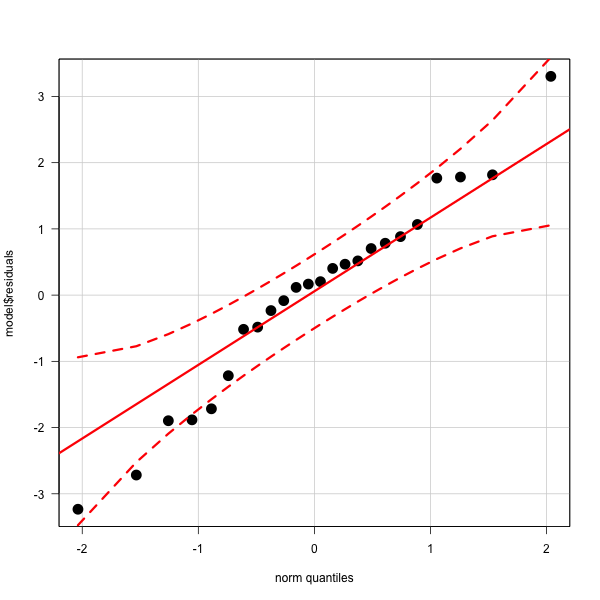
\includegraphics[width=\textwidth]{../img/qq_plot}
  \end{columns}
\end{frame}

\begin{frame}{The normality assumption}{Normality Tests}
  You can also perform statistical tests on the assumption of normality:
  \begin{itemize}
    \item {\bf Shapiro-Wilk;\hfill <- recommended for this course;}
    \item Anderson-Darling;
    \item Lilliefors / Kolmogorov-Smirnov;
  \end{itemize}\bigskip

  These procedures use different aspects of the sample distribution to test the following hypotheses:
  \begin{itemize}
    \item $H_0$: The population is normal;
    \item $H_1$: The population is not normal;
  \end{itemize}\bigskip

  In this case, rejection of the null hypothesis suggests evidence that the {\bf sample} came from a non-normal distribution. Although, for a large enough sample, the CLT might still guarantee a normally distributed {\bf sample mean estimate}, a visual investigation of the distribution of sample's observations is very important in this case.
\end{frame}

\begin{frame}{The independence assumption}
  The strongest assumption used for the t-test is the {\bf independence assumption}. This assumption means that the value of observations are not dependent (biased) on the values of other observations.\bigskip

  Example of independence violation:
  \begin{itemize}
    \item You measure the speed of a robot in 10 trials. However, because the battery is low, the speed will progressively decay;
    \item You measure the accuracy of an algorithm in predicting 20 time series curves. However, 5 of those curves represent different instances of the same model, and are closely related to each other.
  \end{itemize}\bigskip

  In general, we want to guarantee the independence assumption through careful experiment design. The {\bf Durbin-Watson} test can be used to detect auto-correlation, but it is sensitive to the order of observations.
\end{frame}

\section{Conclusion}

\begin{frame}{Conclusion: A framework for statistical testing}
  In this lecture, we introduced the concept of "hypothesis testing" as a way to use data obtained from an experiment to make conclusions about a population. Let's think back to the steps of this procedure:
  \bigskip

  \begin{itemize}
    \item Formulate the question of interest, and define the hypotheses;
    \item Define the minimally interesting effect;
    \item Define desired confidence and power for the test;
    \item Calculate required sample size;\hfill {\bf <- Future Lecture}
    \item Collect the data;
    \item Perform Statistial Analysis, and validate the assumptions;
    \item Draw conclusions and recommendations;
  \end{itemize}
  \bigskip

  In future lectures, we will study variations and special cases of this testing procedure;
\end{frame}

\begin{frame}{Recommended Reading}

  \begin{itemize}
    \item University of Guelph: "Statistical Significance vs Practical Significance: A tutorial."\url{https://atrium.lib.uoguelph.ca/xmlui/bitstream/handle/10214/1869/A_Statistical_versus_Practical_Significance.pdf?sequence=7}

    \item J.T. Mordkoff, "The Assumption(s) of Normality", 2016 \url{http://www2.psychology.uiowa.edu/faculty/mordkoff/GradStats/part\%201/I.07\%20normal.pdf}
  \end{itemize}

\end{frame}
